\chapter{Methods and Implemented Modules}\label{methods-and-implemented-modules}

Chapter~\ref{system-architecture} described \emph{what} the pipeline is. This chapter is about \emph{how} each part works: the data it learns from, the two classifiers, the context modules layered on the second one, and the rules used to judge all of them. Every configuration value, model name, and threshold appears here, so each result can be traced back to the settings that produced it. The order follows the path a message takes, from the model that sees it first to the agents that argue over the hard cases.

\section{Overview}\label{overview}

Static models are far faster than language models. That single fact sets the shape of the method: Tier-1, the static model, handles the bulk of the traffic quickly, and the slow model is called in only for the cases that need more care.

What the slow model brings is context, which is exactly what the fast one lacks. Before it runs, that context is assembled in four ways, each built as its own module and each measured on its own: memory of what a user has done before, retrieval of similar past cases, a curated knowledge base, and a multi-agent chain that splits the decision across four specialised agents.

Because they sit behind a common interface, they can be switched on one at a time. That is what makes the comparison in Chapter~\ref{evaluation-and-results} a fair one rather than a tangle of confounded changes.

The chain is the same one the architecture used: question, requirement, choice, test. Where a section answers to a particular research question that is noted at its head, and the summary table in Chapter~\ref{evaluation-and-results} closes the loop for all three. Section~\ref{reproducibility-summary} then gathers every parameter named anywhere in this chapter into one table, so nothing has to be hunted for.

\section{Datasets}\label{datasets}

The project uses two datasets, and they do different jobs. One trains the fast classifier. The other tests the whole pipeline.

\textbf{Dataset A : the training corpus.} The training corpus holds 52,972 labelled comments merged from three established sources: Davidson et al., contributing 24,783 rows of informal, slang-heavy social media text \citep{davidson2017}; HateXplain, 19,229 rows with human rationales resolved by majority vote \citep{hatexplain2021}; and ToxiGen, 8,960 machine-generated rows carrying implicit, non-obvious toxicity \citep{toxigen2022}. The merge is deliberate, since each corpus covers a weakness the others leave open. Trained on all three, the model sees explicit slurs, subtle implicit hate, and everyday slang instead of one flavour of the problem. Labels are the three classes introduced in Chapter~\ref{state-of-the-art} (hate, offensive, and normal), and text is truncated at 128 tokens. That length was not arbitrary: it already covers the 95th percentile of comment lengths (Figure~\ref{fig:class-distribution}), so cutting there costs almost nothing.

\textbf{Dataset B : the evaluation benchmark.} Metrics come from a separate hand-labelled benchmark, not from held-out training data. The reason is that the object under test is the \emph{pipeline in context}, not a classifier on data resembling its own. So the benchmark is drawn from live records and labelled by hand into the same three classes. How those records were picked matters for reading the results, and it belongs here rather than in Chapter~\ref{evaluation-and-results}.

Drawing them at random would have been the simpler course, and it would have left almost nothing to measure. Toxic messages are thin on the ground in collected traffic to begin with, and thinner still because both platforms let a channel stop the worst of them before viewers see them. YouTube can hold the messages its system flags until the channel approves them, and Twitch's AutoMod holds flagged messages for moderator review, while a short chat delay, set in seconds, gives moderators time to remove a message before it appears \citep{youtubelivechat2026, twitchapi2026}. A pipeline that reads chat as a viewer never receives those messages. Section~\ref{limitations} takes up what that costs the study as a whole. The benchmark carries its own evidence for it: of the two hundred-odd records taken at random, not one proved toxic once a human had read it.

The selection is therefore weighted. Records are scored for how much they are worth labelling by hand, with weight given to three things: a toxic Tier-1 prediction, a disagreement between the two tiers, and low Tier-1 confidence. The sampler reserves a quarter of its quota for records taken at random from the confidently-normal majority and fills the rest from the top of that ranking, so the judge is also scored on cases it ought to leave alone. In the finished benchmark that random share came to 204 of the 1,748 records. Weighting is what put eighty positives in the set at all, and it is the same choice that stops the set standing in for ordinary traffic. What it could not remove is the rarity of toxic content itself, and that rarity is why raw accuracy is set aside in favour of toxic-class metrics, as Section~\ref{evaluation-methodology} explains.

\begin{figure}[H]
\centering
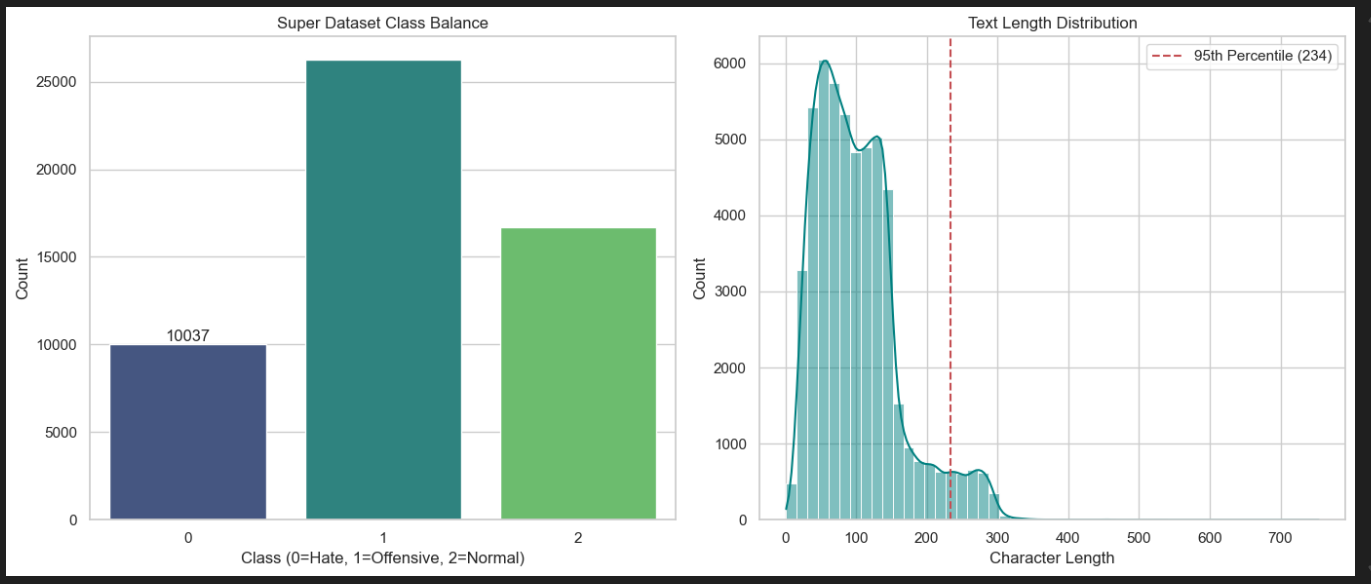
\includegraphics[width=1\linewidth,height=0.85\textheight,keepaspectratio]{figures/class_distribution.png}
\caption{Dataset A. Left: the three-class balance of the 52,972-message training corpus (offensive is the majority class, hate the smallest). Right: the character-length distribution, with the 95th percentile at 234 characters, which is why inputs are truncated at 128 tokens with almost no loss.}\label{fig:class-distribution}
\end{figure}

\section{Tier-1: the fast static classifier}\label{tier-1-the-fast-static-classifier}

\emph{Two questions meet here. Tier-1 has to be quick enough to carry RQ1's real-time claim, and wrong in the particular way that leaves RQ2 something worth correcting.}

Speed is the constraint this model is chosen around, because it has to keep up with a live stream.

\textbf{Classical baselines.} Two simpler models set the bar. A Logistic Regression and a linear SVM, both over TF-IDF features, trained on all 52,972 messages, split 80/20 with a fixed random seed. They are cheap, need no GPU, and land at 75.6 and 75.0 per cent accuracy on the 10,595 held-out messages. Their real value is as a control: they show how far plain word-counting gets, and therefore how much the transformer actually adds. Where they fail is any case that turns on meaning rather than vocabulary, a reclaimed slur used affectionately, or sarcasm that inverts what the words say, because a bag of TF-IDF weights has no way to represent ``this word means the opposite of what it usually does here.''

\textbf{DistilBERT.} The chosen Tier-1 model is a fine-tuned \texttt{distilbert-base-uncased}, a six-layer distilled transformer that keeps most of BERT's language understanding at a fraction of its size and latency \citep{distilbert2019}.

The choice was as much about hardware as about the model, and the arithmetic is worth showing rather than asserting. Everything here was trained and run on a laptop with 12 GB of system memory and a GPU carrying 4 GB of video memory. The fine-tuned Tier-1 model holds 67.0 million parameters across six layers and takes about 269 MB on disk. BERT-base, and with it HateBERT, which keeps BERT's architecture, holds 110 million across twelve layers, roughly 1.6 times as many. Fine-tuning costs more than the weights, though: it needs the weights plus their gradients, plus the optimiser's two moment estimates per parameter, plus the activations held for the backward pass. The working requirement is several times the model size, and at that multiple the larger encoder leaves no workable headroom in 4 GB. The same ceiling is why the training batch size is 8 rather than the conventional 32.

Training itself is unremarkable: two epochs, weight decay 0.01, 100 warm-up steps, and sequences padded and truncated to 128 tokens, with the optimiser and learning rate left at the library defaults of AdamW and 5e-5. To keep fine-tuning time manageable on the laptop GPU, DistilBERT was trained on a random sample of 43,000 of the 52,972 messages rather than on all of them, split 80/20 into 34,400 for training and 8,600 for evaluation. That split was drawn without a fixed seed, so its exact partition cannot be regenerated. Appendix~\ref{hardware-and-software-environment} lists the full environment.

On its 8,600 evaluation messages the model reaches about 79 per cent accuracy and F1 around 0.80, a few points above the classical baselines. Because the baselines were scored on a different held-out set, that gap is indicative rather than exact. The like-for-like comparison is the set of 500 live messages described below, which all three models labelled: on the toxic class, DistilBERT reaches an F1 of 0.38, against 0.27 for Logistic Regression and 0.24 for the SVM. But accuracy is not why it was picked. Latency is. DistilBERT labels a message in roughly 31 milliseconds on this hardware (Section~\ref{latency-and-computational-cost}), which is what lets it sit in front of a live stream without adding lag anyone would notice (throughput is measured in Section~\ref{throughput-scalability}).

Each prediction is a soft-max over the three classes. The highest-scoring class becomes the label, and its probability is the \emph{confidence} that decides whether the second tier is needed (Section~\ref{tier-2-the-llm-judge}).

Figure~\ref{fig:bert-confusion} shows the model's real weakness, and it is the whole reason a second tier exists. The set is 500 messages from a single YouTube stream, labelled by hand and collected separately from the Chapter~\ref{evaluation-and-results} benchmark. DistilBERT gets almost all the normal traffic right, 435 of 452. Then it collapses on the toxic classes. Of 25 genuinely offensive messages it calls 23 of them normal, and it scatters the hate class across all three labels. A model this blind to toxicity in context is a useful fast filter and nothing more, which is exactly the role it is given.

\begin{figure}[H]
\centering
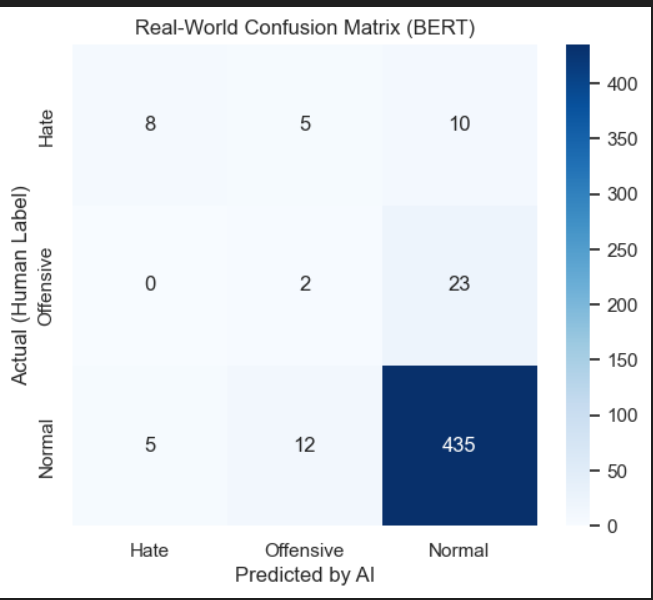
\includegraphics[width=0.9\linewidth,height=0.85\textheight,keepaspectratio]{figures/bert_confusion_matrix.png}
\caption{DistilBERT confusion matrix on 500 hand-labelled messages from one YouTube stream (actual human label vs.~predicted). The model handles normal content well but misreads most toxic messages as normal, motivating the Tier-2 judge.}\label{fig:bert-confusion}
\end{figure}

\section{The Context Agent}\label{the-context-agent}

Before a message is classified at all, the pipeline works out what kind of place it came from.

The naive way would be to hand the model a fixed menu of categories and make it choose. That turns discovery into guesswork the moment a stream fits nothing on the menu. So the Context Agent does the opposite: it asks an LLM to read the stream's metadata, its title, channel, and description, and describe in free text what the stream is about and how strictly it should be moderated. A live esports final comes back as gaming, low strictness, because aggression is expected there. A political broadcast comes back high.

That free-text answer is then normalised onto a stable set of canonical domains (Figure~\ref{fig:context-agent}) so the downstream analytics stay consistent, and the model's original wording is kept beside it. Keeping the raw proposal matters twice over. It is auditable, and it is itself a finding, a record of the categories the model reached for unprompted, including ones outside the seed list. On the benchmark those are common: 628 of the 1,748 records, 36 per cent, carry a domain the seed list did not contain. If the LLM call fails, the agent falls back to safe defaults instead of blocking ingestion, so a hiccup in the reasoning layer never stops the stream.

There is a further consequence, and it is the reason this design was chosen over a fixed list. The canonical domains live in an operator-editable file, \texttt{config/taxonomy.yaml}, not in the code, and every off-list proposal is logged rather than discarded. When a new game, a new platform, or a fresh piece of slang starts appearing, an operator watches it accumulate in those logs and promotes it into the taxonomy without touching a line of Python. The system's sense of context can therefore follow trends as they emerge, which matters a great deal in a setting where the vocabulary of both ordinary speech and abuse keeps shifting. A taxonomy frozen at training time would be stale within months. This one grows with the platforms it watches, and that adaptability is part of what the ``agentic'' claim is meant to deliver.

\begin{figure}[H]
\centering
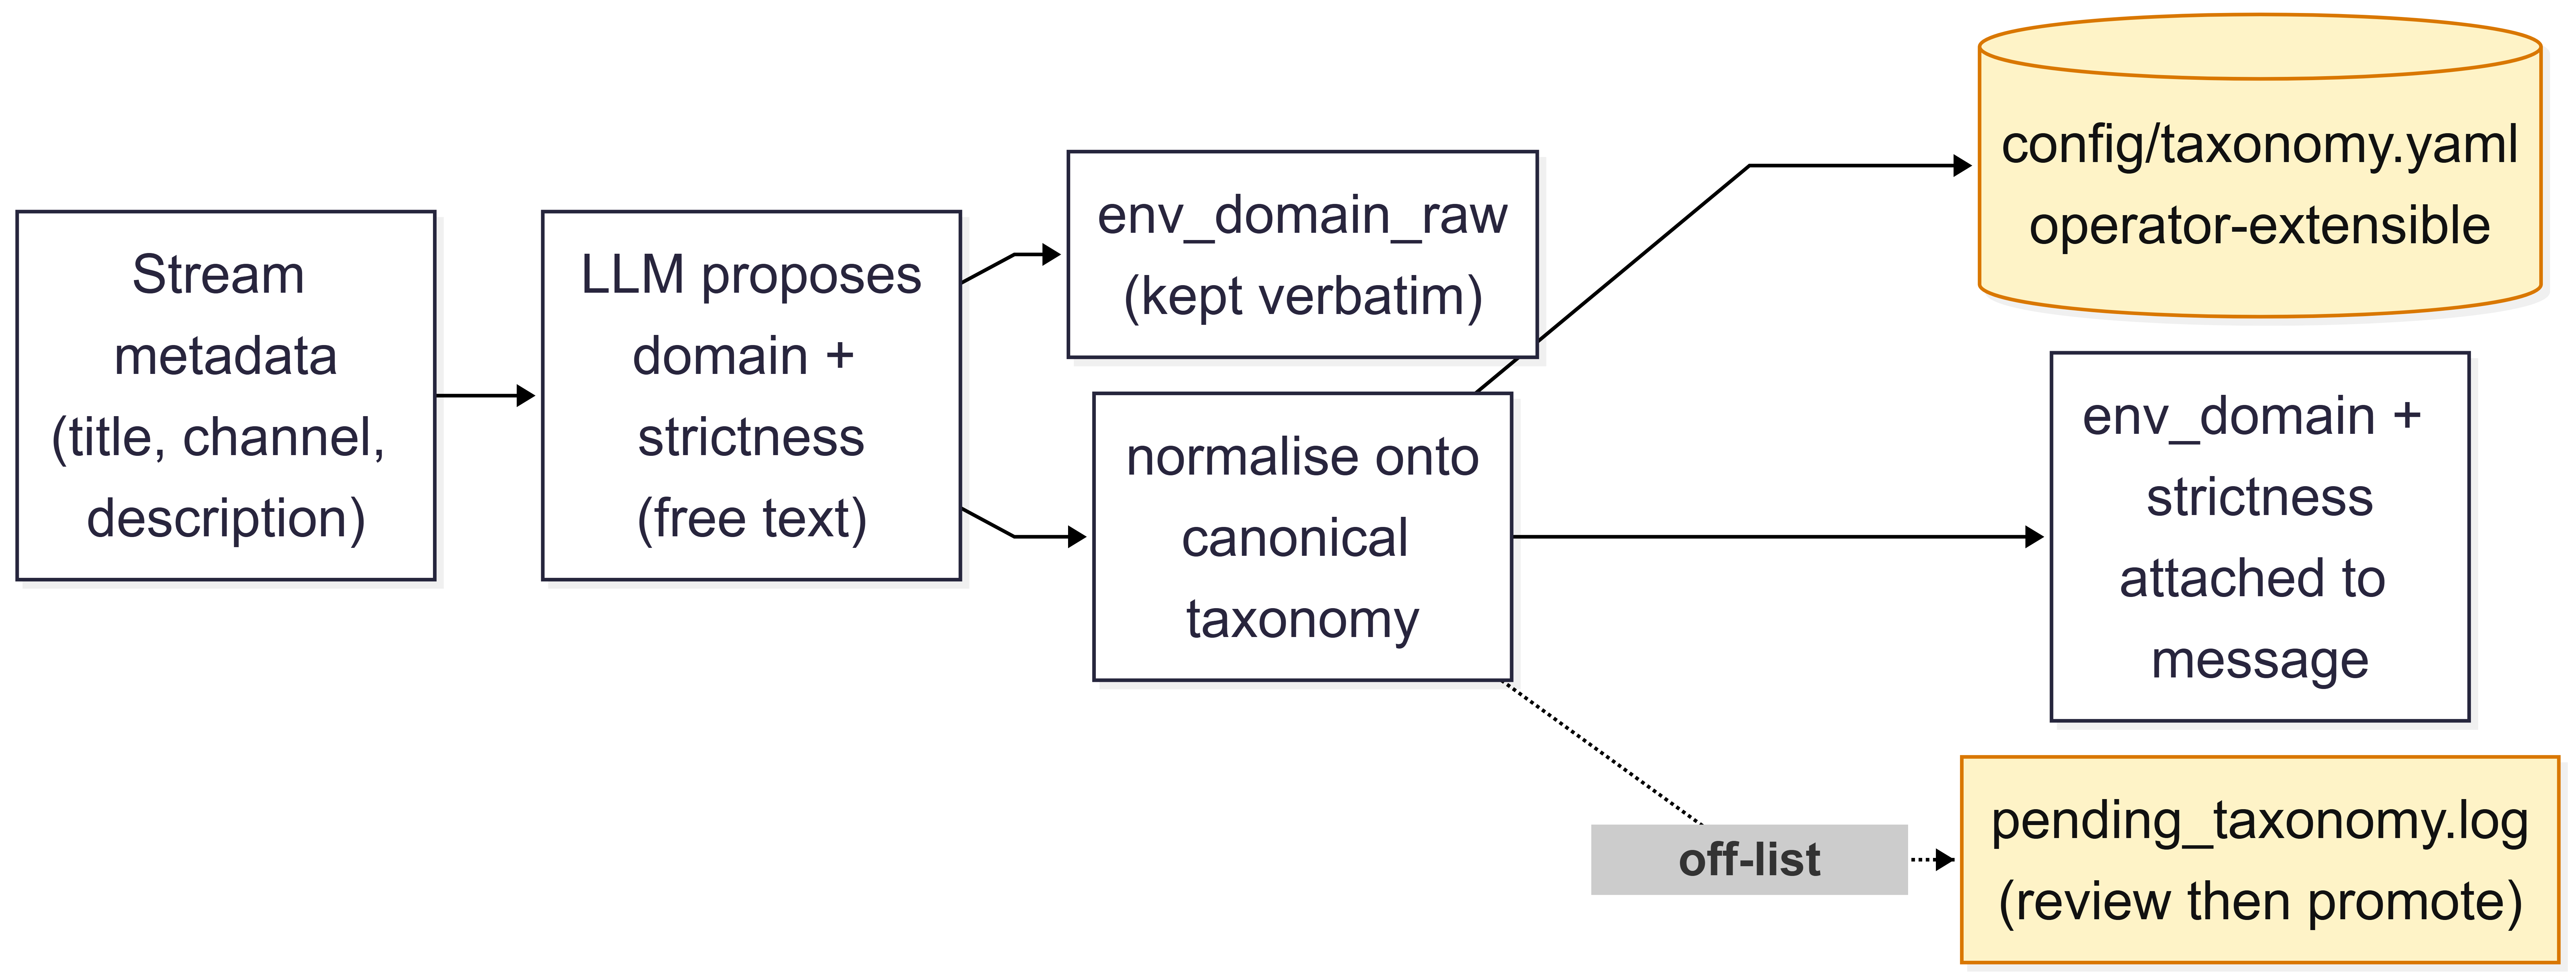
\includegraphics[width=0.9\linewidth,height=0.85\textheight,keepaspectratio]{figures/contextAgent.png}
\caption{The Context Agent: agentic discovery of domain and strictness, then normalisation onto the operator-extensible taxonomy.}\label{fig:context-agent}
\end{figure}

\section{Tier-2: the LLM judge}\label{tier-2-the-llm-judge}

The second tier is where context finally enters the decision. It is a large language model, \texttt{gpt-oss:120b}, an open-weight mixture-of-experts model with 116.8 billion parameters, of which 5.1 billion are active for any one token \citep{gptoss2025}, reached through Ollama under the tag \texttt{gpt-oss:120b-cloud} and used as a judge in the sense of the LLM-as-a-judge literature \citep{llmjudge2023}. The experiments here reach it on Ollama's hosted endpoint, since a model that size will not fit a 4\,GB GPU, but the same interface serves a fully local model such as \texttt{dolphin-llama3} unchanged where the hardware allows.

What it does is narrow. It reads the message, the Tier-1 verdict and its confidence, and the stream's context, then returns one of three verdicts, that Tier-1 was correct, that it was a false positive, or that it was a false negative, along with a written explanation.

Two choices make it behave like a classifier instead of a chatbot. Inference is pinned to temperature zero, so the same input gives the same verdict as nearly as a hosted endpoint allows, since its batching and hardware sit outside the pipeline's control. And the model must return structured JSON, so its output parses without guesswork, with one automatic retry if it ever strays. The explanation is not decoration. It is what lets a human moderator see the reasoning behind an overturned decision, which a bare probability from Tier-1 could never provide.

The judge, on the other hand, is expensive, so it is rationed. It runs only on messages Tier-1 was unsure about, confidence below 0.80, and it runs asynchronously (Figure~\ref{fig:two-tier}), reading its work from storage rather than sitting in the live path. The effect is the one the whole architecture is built around: the model that takes seconds never touches the model that takes milliseconds. It is the difference between answering every email the moment it lands and setting the awkward ones aside for a batch later. The inbox never backs up because of the slow ones. That is the deployed behaviour; the single place where the evaluation departs from it is recorded in Section~\ref{evaluation-methodology}.

One thing about that threshold should be said plainly. The 0.80 figure is a design parameter, not a tuned one. It was fixed before any evaluation, as a round value that pushes clearly-uncertain cases upward while leaving the confident majority alone, and no sweep across candidate thresholds was run to find the value that maximises any particular metric. Which direction the trade runs is easy enough to see: lower the gate and the judge reviews less traffic and misses more of the hard cases, raise it and the reverse happens at greater cost. Where that curve actually turns is left open. Answering it properly would take a calibration study across a range of thresholds, measuring cost against toxic-class recall at each, and that is a study this thesis does not attempt.

Every prompt used here is reproduced verbatim in Appendix~\ref{prompt-library}.

\begin{figure}[H]
\centering
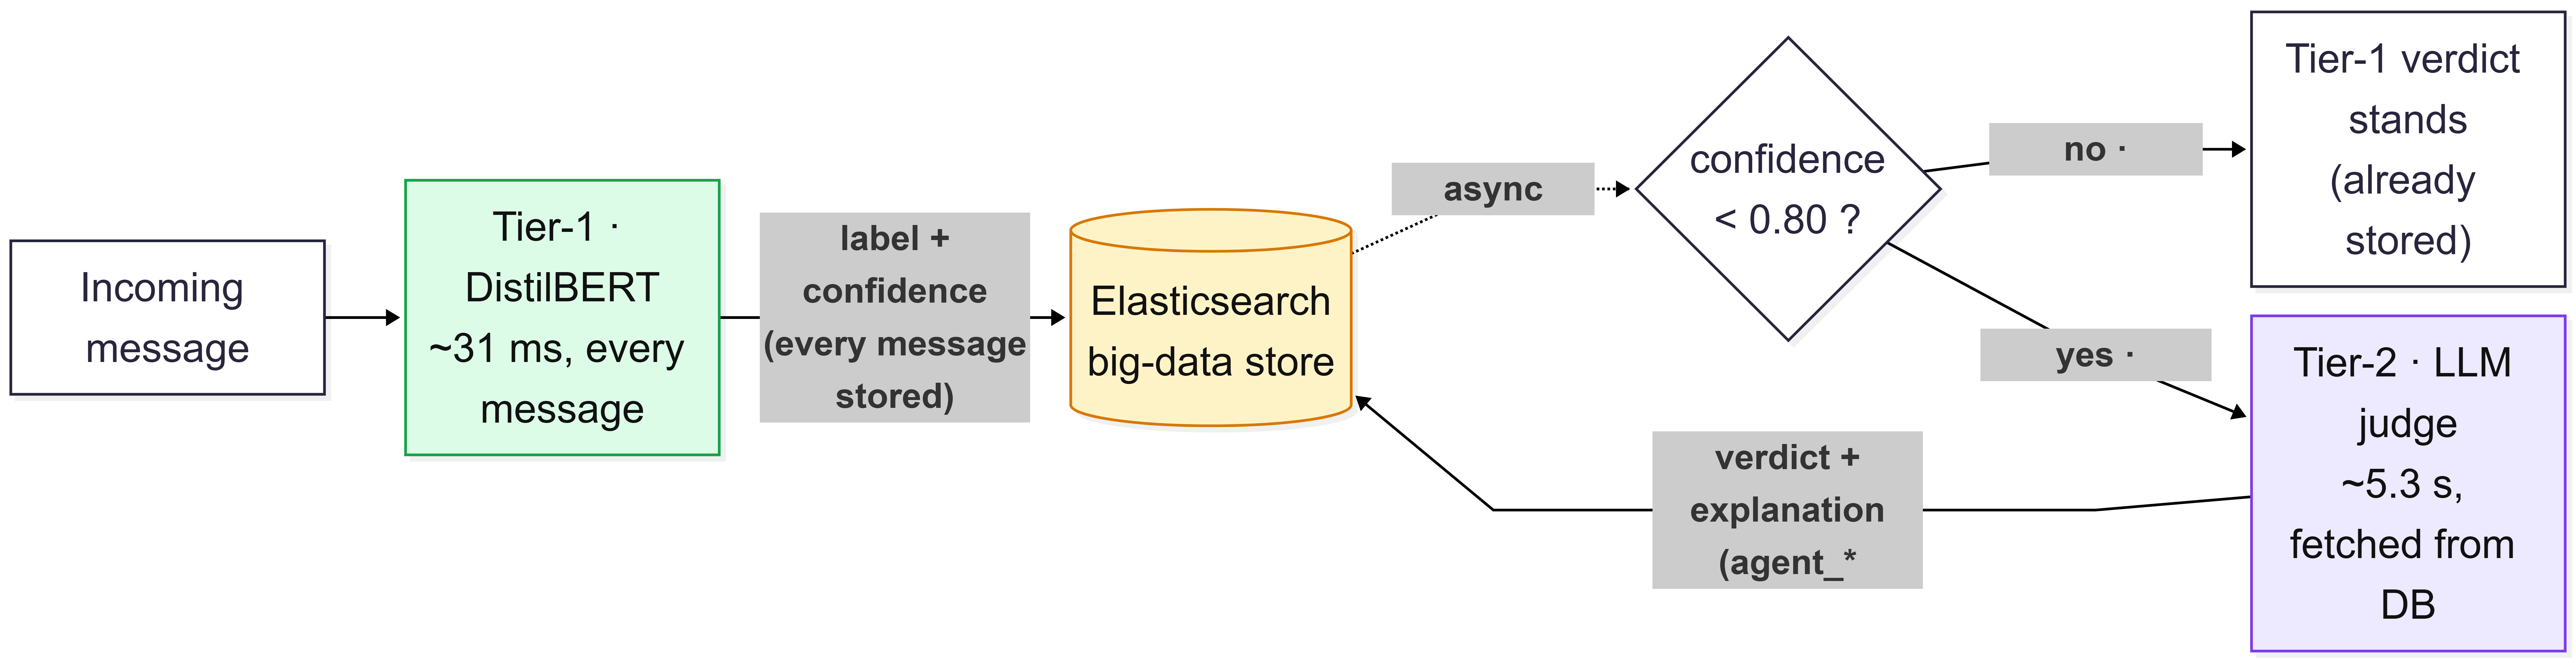
\includegraphics[width=0.95\linewidth,height=0.85\textheight,keepaspectratio]{figures/two_tier_flow.png}
\caption{The two-tier design: a fast static classifier with a confidence gate that escalates only the uncertain minority to the slow LLM judge, asynchronously.}\label{fig:two-tier}
\end{figure}

\section{Temporal memory}\label{temporal-memory}

\emph{The next four sections take the context mechanisms in turn. Each is built to be switched off without disturbing the others, which is what lets RQ3 be answered module by module instead of in aggregate.}

A single message is thin evidence. The same three words can be a shrug or a threat depending on who typed them and what came just before, and Tier-2 on its own sees only the isolated line.

The memory module fixes that by pulling three things out of storage before the judge decides (Figure~\ref{fig:temporal-memory}): the author's recent messages, the last few messages in the same thread, and a short behavioural fingerprint summarising how often that author has been normal, offensive, or hateful lately.

The intuition behind it is ordinary. A regular who has posted a hundred harmless messages and then writes something borderline is probably joking. The same line from an account flagged twice this week reads differently. A moderator who knew both histories would treat them differently, and memory gives the judge that history.

It is bounded on purpose, so the prompt stays a sensible size and old behaviour does not drown out the present. The judge sees the author's last ten messages from the past twenty-four hours, the five messages that came just before this one in the same thread, and a fingerprint computed over the author's last twenty labelled messages from the same twenty-four hours. All four windows are configuration values rather than constants in the code, so any of them can be widened or narrowed without touching the pipeline.

\begin{figure}[H]
\centering
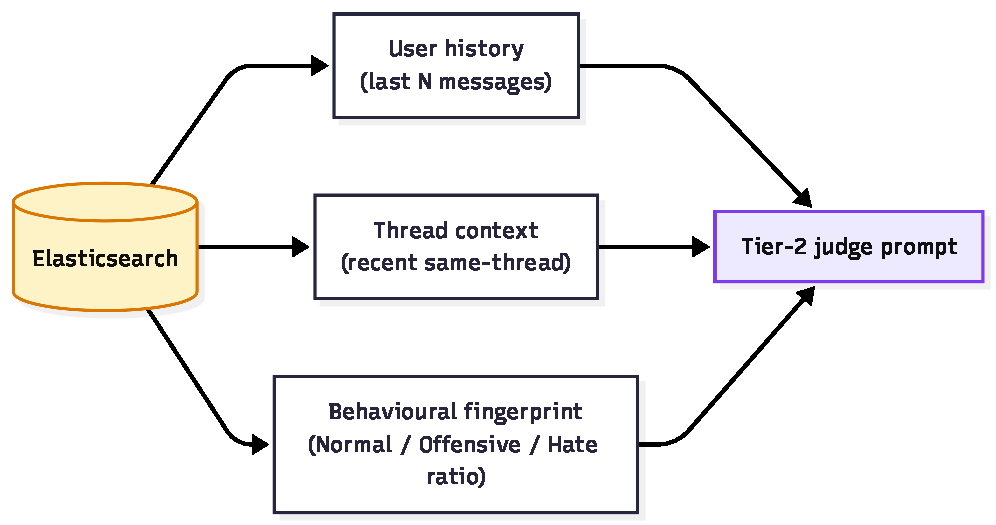
\includegraphics[width=0.9\linewidth,height=0.85\textheight,keepaspectratio]{figures/temporal_memory.pdf}
\caption{Temporal memory: the user history, thread context, and behavioural fingerprint pulled from Elasticsearch into the judge prompt.}\label{fig:temporal-memory}
\end{figure}

\section{Retrieval-augmented moderation (RAG)}\label{retrieval-augmented-moderation-rag}

Memory looks at the \emph{author}. Retrieval looks at \emph{other, similar cases}.

The RAG module embeds the current message into a 384-dimensional vector using a compact sentence-transformer, \texttt{all-MiniLM-L6-v2} \citep{sbert2019}, then asks a Qdrant vector database for the five past messages whose vectors sit closest by cosine similarity, keeping only those above 0.55. Those nearest cases, with the verdicts they received, go to the judge as precedent, following the retrieval-augmented pattern \citep{rag2020}.

Think of it as case law. Faced with an ambiguous message, the judge is shown how comparable messages were handled before, and can lean on that consistency instead of deciding from scratch each time. For evaluation the retrieval is leave-one-out, so the current message is always excluded from its own results and can never retrieve itself to inflate the score. The embedder, the neighbour count of five, and the 0.55 threshold all live in one file, \texttt{config/rag.yaml}, so swapping the embedder is a one-line change.

\section{The LLM-Wiki backend and the switchable interface}\label{the-llm-wiki-backend-and-the-switchable-interface}

RAG grounds the judge in past \emph{cases}. The LLM-Wiki grounds it in curated \emph{knowledge}. Setting those two against each other is one of the experiments this thesis was built to run.

Where RAG retrieves whatever the corpus happens to hold, the Wiki reads from a small hand-written knowledge base: a core policy page defining the three labels; rule pages for gaming, for politics and news, and for reviews, with a general page for every other domain; a glossary of coded language and evasion tricks; and a set of edge-case rulings covering reclaimed slurs, sarcasm, and quoting without endorsing. For any given message the module always supplies the core policy and that message's domain page, then adds the most relevant glossary or edge-case entries, found using the same embedder RAG uses. Keeping the encoder identical was deliberate. Both backends then judge relevance the same way, so the main difference between them is \emph{what} gets retrieved, curated rules or past examples, and that keeps the comparison as clean as two different corpora allow.

That decision is also where this implementation parts company with the pattern it borrows. At the scale Karpathy describes, a hundred or so sources, the wiki needs no retrieval at all: an index page tells the model which files to open and they go straight into the context window, with search recommended only once a collection outgrows that \citep{karpathy2026llmwiki}. The knowledge base here is smaller still, so loading it directly would have served perfectly well. It is indexed anyway, and the reason is methodological rather than technical. Reading the pages straight into the prompt would have changed two variables at once, the corpus and the means of reaching it, leaving no way to attribute any difference in the results to either. Reusing RAG's encoder holds the means of retrieval constant, so the corpus is the main thing that varies, although each backend keeps its own count and cut-off. The knowledge base's eight content pages are split at every second-level heading into 34 entries, a ninth page serving only as navigation and carrying no knowledge of its own. Those entries are embedded once with the same MiniLM encoder and held in memory, and a query returns the four most relevant above a cosine similarity of 0.15, on top of the policy and domain pages that are always included. Those values live in \texttt{config/wiki.yaml}. The threshold sits well below RAG's 0.55 on purpose, because a policy page is relevant to a message in a much looser sense than a near-duplicate past case is, and holding both to the same bar would starve the Wiki of anything to say.

Each is good at a different kind of case. A coded phrase like a ``great replacement'' dog-whistle rarely has a close neighbour among past messages, so RAG may return nothing useful, while the Wiki's glossary names it outright. The trade runs the other way for a message whose meaning lives in one very specific prior case that no policy page anticipated.

Both sit behind a single interface, \texttt{retrieval.py}, and one configuration flag, \texttt{RETRIEVAL\_BACKEND}, picks between them (Figure~\ref{fig:retrieval-backends}): \texttt{rag}, \texttt{wiki}, or \texttt{none}. Switching the live pipeline from vector retrieval to the knowledge base is one line, with nothing else touched. That is the concrete meaning of the switchable backend this thesis claims. A graph-structured variant, GraphRAG, is left as future work.

\begin{figure}[H]
\centering
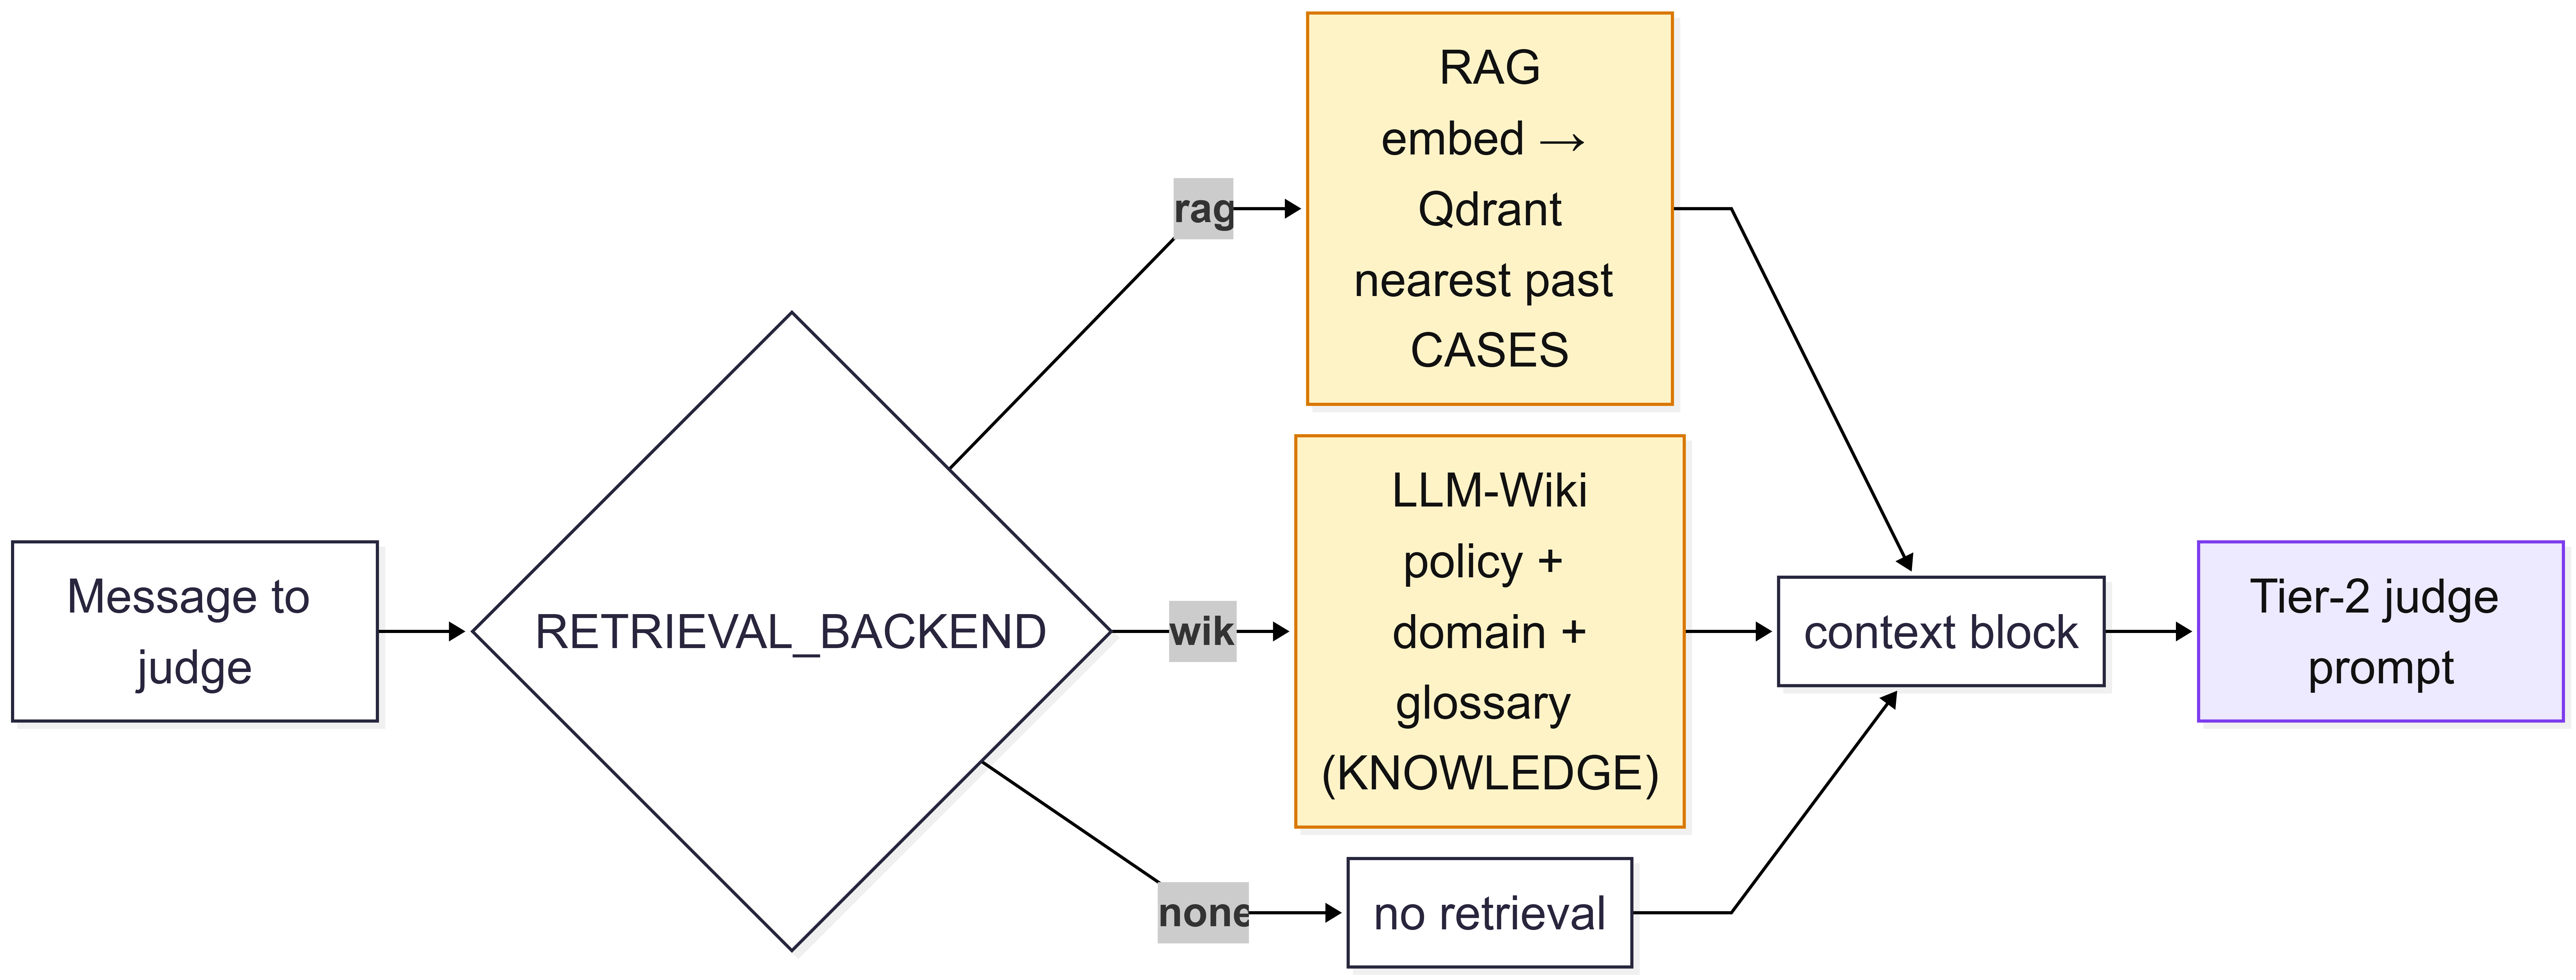
\includegraphics[width=0.9\linewidth,height=0.85\textheight,keepaspectratio]{figures/retrieval_backends.png}
\caption{The switchable retrieval backend: a single flag selects RAG (nearest past cases) or the LLM-Wiki (curated knowledge), feeding the same judge prompt slot.}\label{fig:retrieval-backends}
\end{figure}

\section{The multi-agent chain}\label{multi-agent-decomposition}

So far the judge is one call doing everything at once: reading the content, weighing the author, deciding. The multi-agent chain breaks that into four smaller calls, each with a narrow job, run in sequence (Figure~\ref{fig:multi-agent}).

\begin{enumerate}
\def\labelenumi{\arabic{enumi}.}
\tightlist
\item \textbf{Risk Scorer} reads only the message content and rates its toxicity from 0 to 1, with no knowledge of who sent it.
\item \textbf{Behaviour Profiler} reads only the author's history and rates the account low, medium, or high risk, with no knowledge of the current message.
\item \textbf{Escalator} takes those two signals and decides how to route the case (clear it automatically, flag it automatically, or send it to a human).
\item \textbf{Supervisor} reads everything the others produced and issues the final verdict in the same three-way format as every other variant (Tier-1 correct, false positive, or false negative), so it stays directly comparable.
\end{enumerate}

Why split a job one prompt could do? For the same reason a newsroom separates the reporter from the editor. When one person does both, a mistake afterwards is impossible to place, in the facts or in the judgement. Separate the steps and each one leaves a record. If the final verdict is wrong, the stored risk score, behaviour rating, and routing decision show which step went astray, and that per-step trace is what the dashboard's Multi-Agent tab displays and what Section~\ref{inside-the-multi-agent-chain} analyses. The cost is four LLM calls per message instead of one, which is affordable only because, like the rest of Tier-2, this runs on the flagged minority alone.

\begin{figure}[H]
\centering
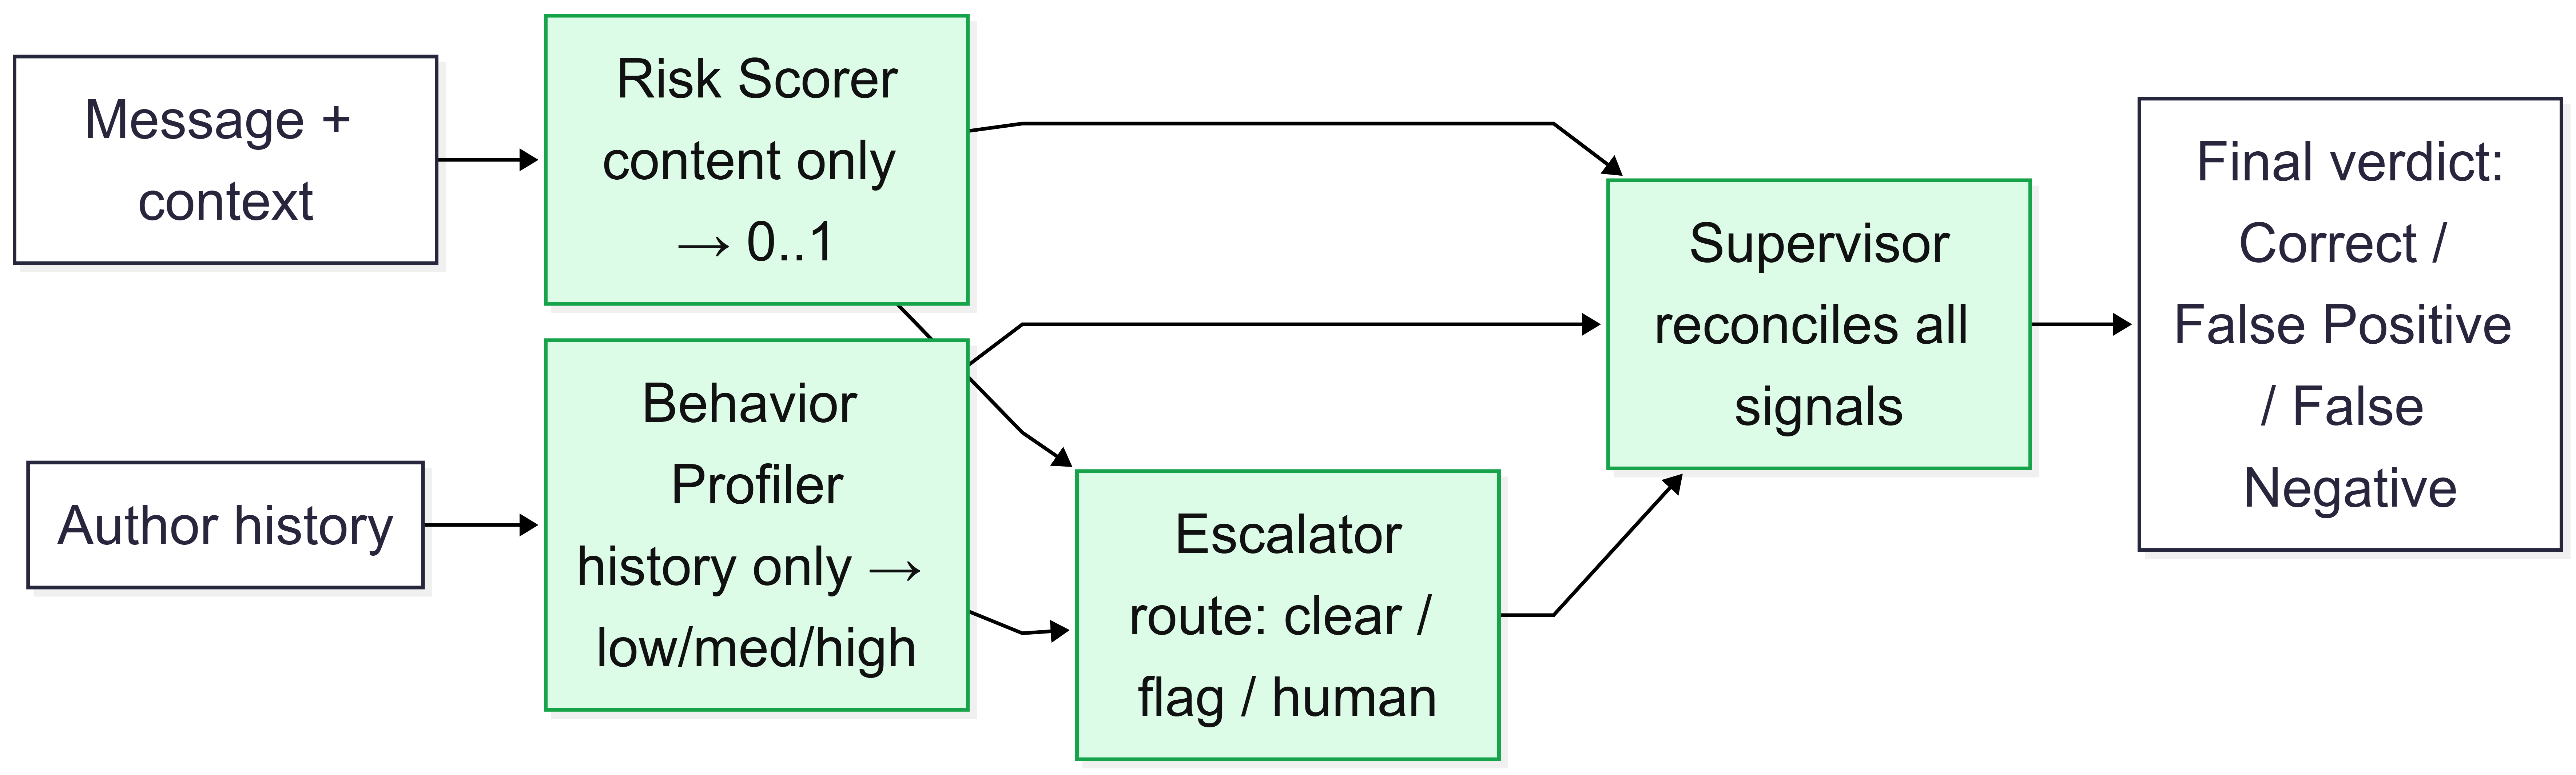
\includegraphics[width=0.9\linewidth,height=0.85\textheight,keepaspectratio]{figures/Multi-agent.png}
\caption{The multi-agent chain: the Risk Scorer and Behaviour Profiler feed an Escalator and a Supervisor that issues the final verdict.}\label{fig:multi-agent}
\end{figure}

\section{Evaluation methodology}\label{evaluation-methodology}

One departure from the live configuration should be recorded before anything else. In deployment the confidence gate decides what the judge ever sees; for the evaluation it was set aside, and every variant judged all 1,748 records whatever Tier-1's confidence had been. That is what lets the configurations be compared on identical rows rather than on whichever subset each happened to receive, and it is also what makes the control group meaningful, since those confident cases are precisely the ones a judge should decline to overturn.

The rest of the method is shaped by one awkward fact: toxic content is rare, in live traffic and in this benchmark alike. A model that labelled everything ``normal'' would score 95.4 per cent accuracy here and catch not one toxic message. Raw accuracy here is not merely unhelpful. It is actively misleading, because reporting it would reward the model for doing nothing.

So the evaluation leads with the toxic class. Every variant is reported with precision, recall, and F1 on hate-plus-offensive content, alongside confusion matrices showing exactly where the errors land, with three-class and binary accuracy kept as secondary figures only. To put the variants on equal footing, their different verdict formats are first mapped to a common label: a ``correct'' verdict keeps Tier-1's label, a ``false positive'' becomes normal, a ``false negative'' becomes toxic. Because a false-negative verdict does not say which toxic class was missed, the three-class accuracy counts it as offensive. A memory verdict and a multi-agent verdict can then be scored the same way against the same ground truth. Finally, since differences between variants can be small on a benchmark holding few toxic cases, each pairwise difference is tested with McNemar's test, in its continuity-corrected form, the standard paired test for two classifiers on one dataset \citep{mcnemar1947, dietterich1998}. McNemar's test counts every verdict, so it measures overall correctness, which the normal majority dominates; the toxic-F1 difference is therefore also given a paired bootstrap confidence interval \citep{efron1993}. Together they are what separate a real improvement from a lucky one, and it runs throughout Chapter~\ref{evaluation-and-results}.

\section{Summary of settings and parameters}\label{reproducibility-summary}

The settings behind the results appear above, next to the arguments that motivate them. Table~\ref{tab:params} gathers all of them in one place, so no setting has to be hunted for in the chapter or in the source. Where a value was forced by the hardware or chosen for a particular reason, the text gives that reason, and library defaults are named as such. None of the thresholds, though, were arrived at by sweeping a range and keeping whichever score came out highest. They are design settings, the confidence gate and the two retrieval cut-offs alike, and the text says so where each is introduced.

Three things complete the picture. Every prompt, for the Context Agent, the judge, and each of the four agents, appears verbatim in Appendix~\ref{prompt-library}, because a prompt shapes a result as surely as a learning rate does. The hardware and software environment, down to package versions and container tags, is in Appendix~\ref{hardware-and-software-environment}. And the whole stack comes from one \texttt{docker-compose} file, so the same Kafka, Spark, Elasticsearch, and Qdrant start with a single command, after which the evaluation scripts run against the same benchmark file.
\renewcommand{\arraystretch}{1.5} 

\begin{longtable}{@{}
  >{\raggedright\arraybackslash}p{\dimexpr 0.22\linewidth - 1.6\tabcolsep \relax}
  >{\raggedright\arraybackslash}p{\dimexpr 0.30\linewidth - 1.6\tabcolsep \relax}
  >{\raggedright\arraybackslash}p{\dimexpr 0.26\linewidth - 1.6\tabcolsep \relax}
  >{\raggedright\arraybackslash}p{\dimexpr 0.22\linewidth - 1.6\tabcolsep \relax}@{}}
\caption{Every configuration value behind the reported results, with where it is set.}\label{tab:params}\tabularnewline
\toprule
\textbf{Component} & \textbf{Setting} & \textbf{Value} & \textbf{Where set} \\
\midrule
\endfirsthead
\toprule
\textbf{Component} & \textbf{Setting} & \textbf{Value} & \textbf{Where set} \\
\midrule
\endhead
\bottomrule
\endlastfoot

Tier-1 model & base checkpoint & \texttt{distilbert-\allowbreak base-\allowbreak uncased} & \texttt{models/\allowbreak bert\_final} \\
 & training data & random sample of 43,000 of the 52,972 messages & training notebook \\
 & epochs / batch size & 2 / 8 & training notebook \\
 & optimiser & AdamW, lr 5e-5 (both library defaults), weight decay 0.01, 100 warm-up steps & training notebook \\
 & max sequence length & 128 tokens & training and inference \\
 & checkpoint directory & \texttt{models/bert\_final} & \texttt{MODEL\_DIR} \\
 & inference device & CPU by default, GPU selectable & \texttt{DEVICE} \\
 & train/evaluation split & 80/20; seeded for the baselines, unseeded for DistilBERT & training notebook \\
\addlinespace[1em]

Confidence gate & escalate to Tier-2 below & 0.80 (design choice, not calibrated) & processor \\
\addlinespace[1em]

Tier-2 judge & model & \texttt{gpt-oss:120b-\allowbreak cloud} via Ollama & \texttt{OLLAMA\_MODEL} \\
 & temperature & 0 (near-deterministic on a hosted endpoint) & judge call \\
 & output format & structured JSON, one retry on parse failure & judge call \\
\addlinespace[1em]

Temporal memory & author history window & 10 messages & \texttt{MEMORY\_\allowbreak USER\_\allowbreak WINDOW\_\allowbreak SIZE} \\
 & thread context window & 5 messages & \texttt{MEMORY\_\allowbreak THREAD\_\allowbreak WINDOW\_\allowbreak SIZE} \\
 & look-back (author history and fingerprint) & 24 hours & \texttt{MEMORY\_\allowbreak LOOKBACK\_\allowbreak HOURS} \\
 & fingerprint window & 20 messages & \texttt{MEMORY\_\allowbreak FINGERPRINT\_\allowbreak WINDOW} \\
\addlinespace[1em]

RAG & embedding model & \texttt{all-MiniLM-L6-v2}, 384 dimensions & \texttt{config/rag.yaml} \\
 & neighbours retrieved & 5 & \texttt{config/rag.yaml} \\
 & similarity threshold & 0.55, cosine & \texttt{config/rag.yaml} \\
 & self-exclusion & on (leave-one-out) & \texttt{config/rag.yaml} \\
\addlinespace[1em]

LLM-Wiki & embedding model & identical to RAG, by design & \texttt{config/rag.yaml} \\
 & knowledge base & 8 content pages, 34 entries split at second-level headings & \texttt{wiki/} \\
 & always supplied & core policy plus the domain page & \texttt{config/\allowbreak wiki.yaml} \\
 & entries retrieved & 4 & \texttt{config/\allowbreak wiki.yaml} \\
 & similarity threshold & 0.15, cosine & \texttt{config/\allowbreak wiki.yaml} \\
\addlinespace[1em]

Retrieval backend & selector & \texttt{rag} / \texttt{wiki} / \texttt{none} & \texttt{RETRIEVAL\_\allowbreak BACKEND} \\
\addlinespace[1em]

Multi-agent & calls per message & 4, run in sequence & agent chain \\
 & risk score range & 0 to 1, continuous & Risk Scorer \\
 & behaviour rating & low / medium / high & Behaviour Profiler \\
 & routing actions & auto\_clear / auto\_flag / human\_review & Escalator \\
 & failure handling & defaults to \texttt{human\_review} on a parse failure & agent chain \\
\addlinespace[1em]

Kafka & topic / partitions / replication & \texttt{universal\_stream} / 1 / 1 & \texttt{docker-\allowbreak compose.yml} \\
 & retention & 24 hours or 1 GB & \texttt{docker-\allowbreak compose.yml} \\
\addlinespace[1em]

Elasticsearch & index & \texttt{real\_time\_\allowbreak analysis} & \texttt{INDEX\_NAME} \\
\addlinespace[1em]

Qdrant & collection / distance & \texttt{moderation\_\allowbreak records} / cosine & \texttt{QDRANT\_\allowbreak COLLECTION} \\

\end{longtable}
% Reset arraystretch to default for the rest of the document
\renewcommand{\arraystretch}{1.0}

\section{The operator surface: dashboard and analyst chat}\label{the-operator-surface-dashboard-and-analyst-chat}

Everything so far runs without anyone watching. But a moderation system nobody can see into is a system nobody can trust, so the last implemented module is the human side: two Streamlit applications, an operator dashboard and a natural-language chat. Why they were built rather than left to Kibana is answered in Section~\ref{layer-5-context-injection-and-the-analyst-surface}. What follows is what they do.

\textbf{The dashboard} gathers the pipeline into one tabbed console, and every tab answers a question an operator or reviewer actually asks:

\begin{itemize}
\tightlist
\item \textbf{Status strip and Overview} answer ``is it working right now?'' The strip shows, at a glance, whether messages are flowing, how fresh the last record is, and whether Elasticsearch, Qdrant, and Ollama are up; the overview shows volume and the mix of labels. This is the view an operator keeps open during a live event.
\item \textbf{Live Monitor} answers ``what is happening in the stream?'' Label, platform, and domain breakdowns update as messages arrive, so a spike in toxicity during a hate raid is visible as it happens rather than afterwards.
\item \textbf{Record Inspector} answers ``why was this one message decided that way?'' Picking a single record lays out its full trace: the ingest context, the Tier-1 label and confidence, the Tier-2 verdict with its written explanation, the memory bundle, and, for benchmark records, the RAG, Wiki, and multi-agent verdicts. It is the tool for auditing or debugging an individual decision.
\item \textbf{Evaluation} answers ``which configuration is better?'' It renders the per-variant comparison, confusion matrices, and deltas that make up the results of Chapter~\ref{evaluation-and-results}, so the numbers can be inspected live rather than exported.
\item \textbf{RAG} and \textbf{LLM-Wiki} answer ``what context did the judge actually get?'' Each shows the backing store's statistics and lets a reviewer paste a message and watch the retrieval happen, the precedents or the knowledge entries the judge would receive.
\item \textbf{Multi-Agent} answers ``how did the four agents reason?'' It surfaces the risk score, behaviour rating, routing decision, and each agent's rationale behind a verdict.
\end{itemize}

The dashboard assumes a reviewer who knows where to click. \textbf{The analyst chat} assumes one who does not. A moderator types a question in plain language, and a small fixed tool registry turns it into an Elasticsearch query and a written answer. ``How many toxic messages came from Twitch today?'' returns a count. ``Show me the worst offenders'' returns the top users by toxic volume. ``Was this account's behaviour a problem?'' returns a per-user review. ``List the messages the AI wrongly flagged'' returns the false positives. That registry is deliberately small and closed, so the agent can search, aggregate, and audit, and can do nothing at all outside that remit. It is what stops a conversational model from inventing actions it should never take.

Between them the two applications serve both audiences at once: the moderator who has to watch and question a live stream without writing a query, and the researcher or supervisor who has to open up every stage and compare every variant. Two purpose-built applications cover both, which an off-the-shelf dashboard could not do alone.
